\documentclass{article}
\usepackage[utf8]{inputenc}
\usepackage{graphicx}
\usepackage{amsmath}
\usepackage{mathtools}


\title{Laboratorio 3. Oscilaciones de una cuerda tensa}
\author{Carlos Alberto Dagua Conda, Hector Fabio Jimenez Saldarriaga, \\Juan Camilo Castrillón,\thanks{carlosdaguaco@utp.edu.co, hfjimenez@utp.edu.co, jucacastrillon@utp.edu.co} }
\date{March 2016}

\begin{document}

\maketitle

\section{Abstract}
In this paper we will study the oscillations of a stretched string with different configuration of a phenomena, for example, the mass density of a string and tension, in addition we have to explored this laboratory building different relations between parameters and we have concluded about the particular phenomena.

\section{Introduction}

[1] Un movimiento cualquiera que se repite en un periodo constante  de tiempo se le llama “movimiento periódico”. Si un sistema en particular, posee un movimiento periódico, se mueve alternativamente en uno y otro sentido siguiendo la misma trayectoria se le denominara “movimiento oscilatorio o vibratorio ”. Por ejemplo el péndulo de un reloj, una masa suspendida de un resorte y separada de su posición de equilibrio, la cuerda de un instrumento musical, un átomo en una red cristalina a una dada temperatura, etc. representan movimientos oscilatorios.
$\\$
\subsection{Ondas estacionarias}

En un cuerpo de tamaño finito y prácticamente unidimensional, como puede ser una cuerda de longitud L sujeta por sus extremos con una tensión T puede observarse una situación particular: un tren de ondas que viaja por la cuerda en un sentido al llegar a uno de los extremos se refleja, al cabo de un cierto tiempo habrá ondas que viajan en un sentido y ondas que lo hacen en sentido contrario. Estos trenes de ondas se superponen, interfieren, luego habrán punto en los cuales las amplitudes se suman y otros en los cuales se cancelan. Aquellos puntos donde la amplitud es máxima se llaman “antinodos“ y en los cuales la amplitud es nula se llaman “nodos ”[1, 2].\\
Este fenómeno se lo conoce como “ondas estacionarias”.
$\\$
Es característico de una onda estacionaria que la amplitud para distintas partículas de la cuerda dependerá de la posición de cada partícula en particular, de ahí su nombre, es claro por lo tanto que no se transporta energía a lo largo de una onda estacionaria ya que esta no puede fluir a través de los puntos nodales (amplitud nula); podemos decir entonces que la energía permanece “estacionaria”.\\
En una cuerda tensa la elasticidad de la misma dependerá de la tensión T entre sus extremos así como su inercia estará determinada por la relación masa/longitud (densidad lineal $\mu$). En un análisis que aquí obviaremos podemos obtener la velocidad de propagación de una onda en una cuerda tensa:
\begin{equation}
    v=\frac{T}{\mu}
\end{equation}

Tomemos una cuerda de longitud $L$ y densidad lineal $\mu =\frac{m}{L}$ sometida a una tensión $T$ , bajo la condición que en sus extremos haya siempre nodos se deduce fácilmente que la longitud de la cuerda $L$ debe ser un número entero de medias longitudes de onda $(\frac{\lambda}{2})$ entonces:
\begin{equation}
    L=n\frac{\lambda}{2}
\end{equation}

Si se relaciona $\lambda = \frac{v}{f}$ con $(1)$ y $(2)$ se encuentra una expresión que da las frecuencias
características de una onda estacionaria en función de parámetros conocidos $T$, $\mu$ y $L$.
\begin{equation}
    f_{n}=\frac{n}{2L}\sqrt{\frac{T}{\mu}}
\end{equation}

\section{Análisis}
\subsection{Con los datos del ítem 3 del procedimiento:}
$\bullet$ Construya una gráfica de frecuencia $f$ en función del número de armónicos $n$. ¿Qué clase de curva obtiene? ¿Cómo varía la frecuencia en función de los armónicos?
$\\$
$\\$
\emph{Solución}
\begin{figure}[h]
    \centering
    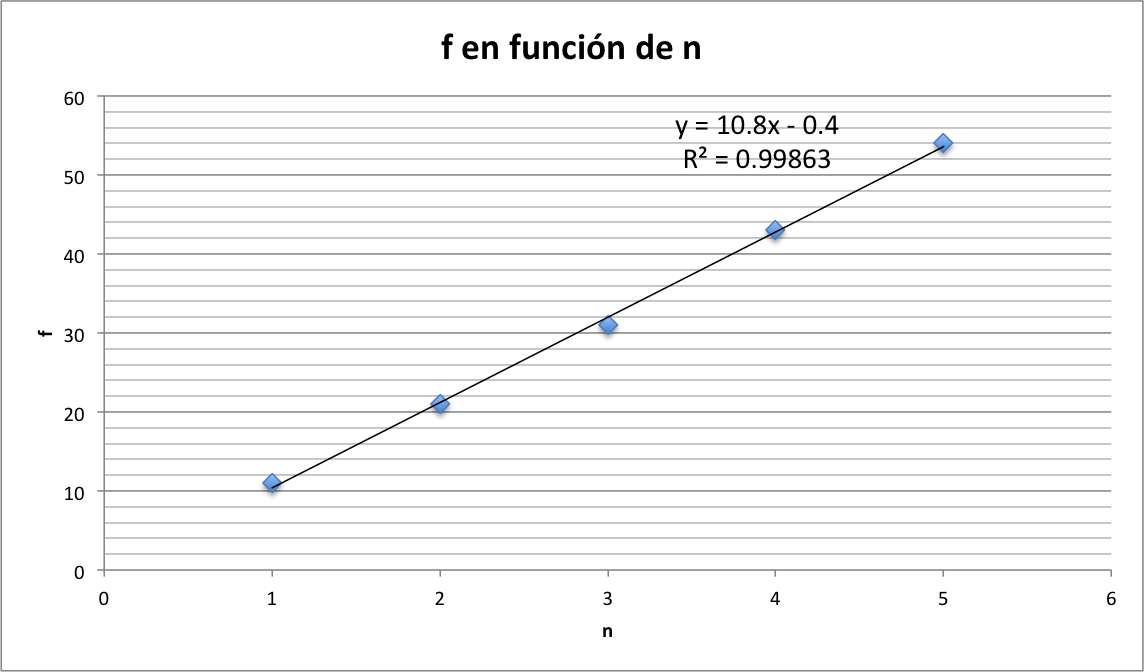
\includegraphics[width=1.0\textwidth]{1.png}
    \caption{Gráfica de la frecuencia en función de el número de armónicos.}
    \label{fig:my_label}
\end{figure}

La clase de curva que se obtiene de construir una gráfica de frecuencia $f$ en función del número de armónicos $n$ es una recta de la forma (\emph{Veáse Figura 1}):
\begin{equation}
    y=mx\pm b
\end{equation}
La frecuencia varía en función de los armónicos de forma directa, es decir, la frecuencia $f$ es directamente proporcional a el número de armónicos $n$, se presenta de la siguente forma:
\begin{equation}
    f\ \ \ \alpha \ \ \ n 
\end{equation}

$\bullet$ Si la gráfica en el numeral anterior es una línea recta, haga el análisis correspondiente para obtener el valor de la densidad de masa $\mu$ (Valor experimental) con su correspondiente incertidumbre.
$\\$
$\\$
\emph{Solución}
\begin{equation}
    f_{n}=\frac{n}{2L}\sqrt{\frac{T}{\mu}}
\end{equation}

\begin{equation}
    y=10.8x-0.4
\end{equation}

Comparando las ecuaciones $(3)$ y $(4)$ se obtiene la siguiente relación:
\begin{equation}
    10.8=\frac{1}{2L}\sqrt{\frac{T}{\mu}}
\end{equation}

Despejando $\mu$ de la ecuación $(5)$ se obtiene que:
\begin{equation}
    \mu=\frac{1}{4L^{2}}\frac{T}{10.8^{2}}
\end{equation}

Para el primer análisis se obtuvieron los valores experimentales directos de la Longitud $(L)$ y de la tensión $(T)$
\begin{equation*}
    L=1.03 (m) \ \ \ \ \ \ T=1.4112 (N)
\end{equation*}
Reemplazando en $(6)$ y realizando un análisis dimensional se obtiene:
\begin{equation}
    \mu=\frac{1}{m^{2}}\frac{\frac{kg m}{s^{2}}}{s^{2}}=\frac{kg}{m}
\end{equation}
\begin{equation}
    \mu=2.85x10^{-03}\pm 0.001\frac{kg}{m}
\end{equation}

$\bullet$ La densidad de la cuerda calculada a partir de su masa y longitud es de $3.7x10^{-03}\frac{kg}{m}$. La masa se midió con una incertidumbre de $\pm0.0001 \ g$ y la longitud con $\pm0.1 \ cm$ Calcule la incertidumbre de la densidad mediante la expresión:
\begin{equation}
\mu=\frac{m}{l_{T}}
\end{equation}
donde $m$ es la masa de la cuerda y $l^{T}$, la longitud total de la cuerda. 
$\\$
$\\$
\emph{Solución:}
\begin{equation}
    \mu=\frac{9.8726x10^{-03}}{2.630}\frac{kg}{m}=3.75x10^{-03}\pm 0.001\frac{kg}{m}
\end{equation}
$\bullet$ Considere esta valor como teórico y compare en términos de porcentaje el valor $\mu$ obtenido en el paso anterior.
$\\$
$\\$
\emph{Solución:}
El valor teórico de la incertidumbre es la ecuación $(10)$ al compara este valor con el obtenido en la ecuación $(8)$ se tiene un Error porcentual de:
\begin{equation}
    \%E=\frac{|3.7x10^{-03}-2.85x10^{-03}|}{3.7x10^{-03}}x100\%=22.97\%
\end{equation}


\subsection{Con los datos de tensión y frecuencia: }

$\bullet$ Construya un gráfico de frecuencia en función de la raiz cuadrada de la tensión. ¿Es su gráfica una línea recta?.
$\\$
$\\$
\emph{Solución:}

\begin{figure}[h]
    \centering
    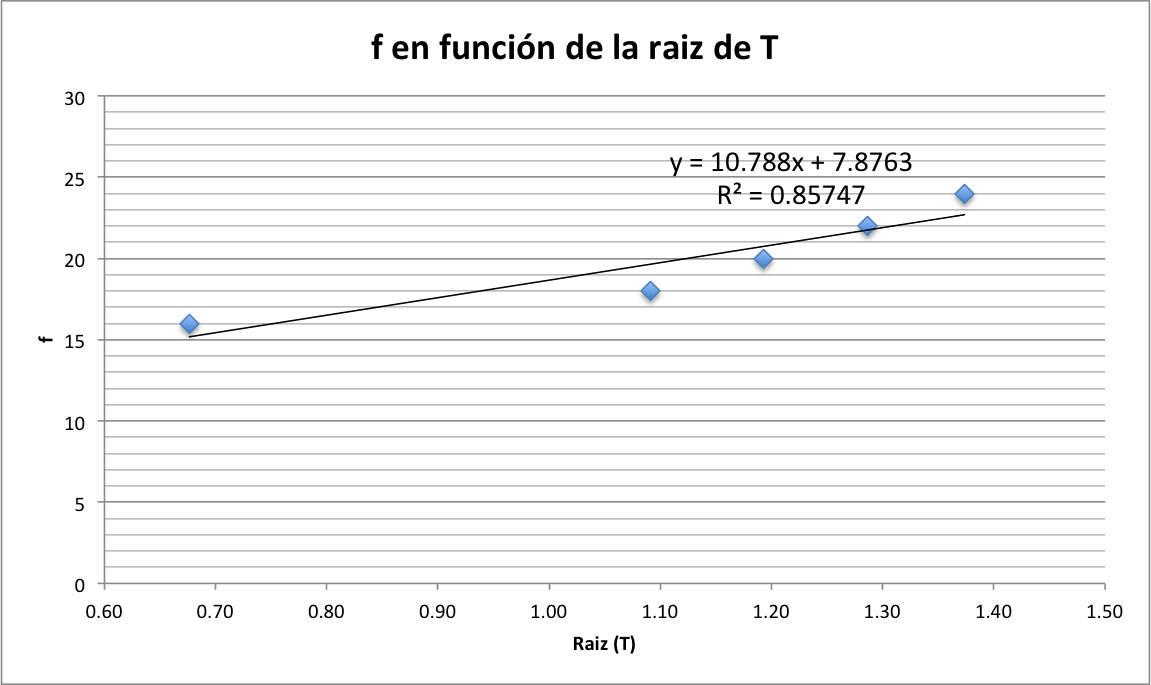
\includegraphics[width=1.0\textwidth]{2.png}
    \caption{Gráfica de la frecuencia en función de la raíz de la tension (T).}
    \label{fig:my_label}
\end{figure}

Al construir una gráfica de la frecuencia en función de la raiz cuadrada de la tensión su gráfica corresponde a una línea recta de la forma que muestra la ecuación $(1) \emph{(Veáse Figura 2)}$. Lo que muestra que la relación entre la frecuencia y la raiz cuadrada de la tensión son directamente proporcionales, es decir:
\begin{equation}
    f \ \ \ \ \alpha \ \ \ \ \sqrt{T}
\end{equation}
$\bullet$ A partir de su gráfico obtenga la ecuación que relaciona la frecuencia con la tensión y de esta ecuación obtenga un nuevo valor para $\mu$ con su respectiva incertidumbre. Compare este valor con el teórico.
$\\$
$\\$
\emph{Solución: }
$\\$
\begin{equation}
    y=10.788+7.8763
\end{equation}

Comparando $(3)$ y $(9)$ se obtiene la siguiente relación:
\begin{equation}
    10.788=\frac{n}{2L}\frac{1}{\sqrt{\mu}}
\end{equation}
\begin{equation}
    \mu=\frac{n^{2}}{4L^{2}}\frac{1}{10.788^{2}}
\end{equation}
Para el segundo análisis se obtuvieron los valores experimentales directos de la Longitud $(L)$ y del segundo armonico $(n)$
\begin{equation*}
    L=1.03 (m) \ \ \ \ \ \ n=2
\end{equation*}
\begin{equation}
    \mu=8.099x10^{-03}\pm 0.0041\frac{kg}{m}
\end{equation}

\begin{equation}
    \%E=\frac{|3.7x10^{-03}-8.099x10^{-03}|}{3.7x10^{-03}}x100\%=118.89\%
\end{equation}


\subsection{Con los datos de longitud y frecuencia: }
$\bullet$ Construya un gráfico de frecuencia $f$ en función de $\frac{1}{L}$. ¿Es el gráfico una línea recta? ¿Por qué?

\begin{figure}[h]
    \centering
    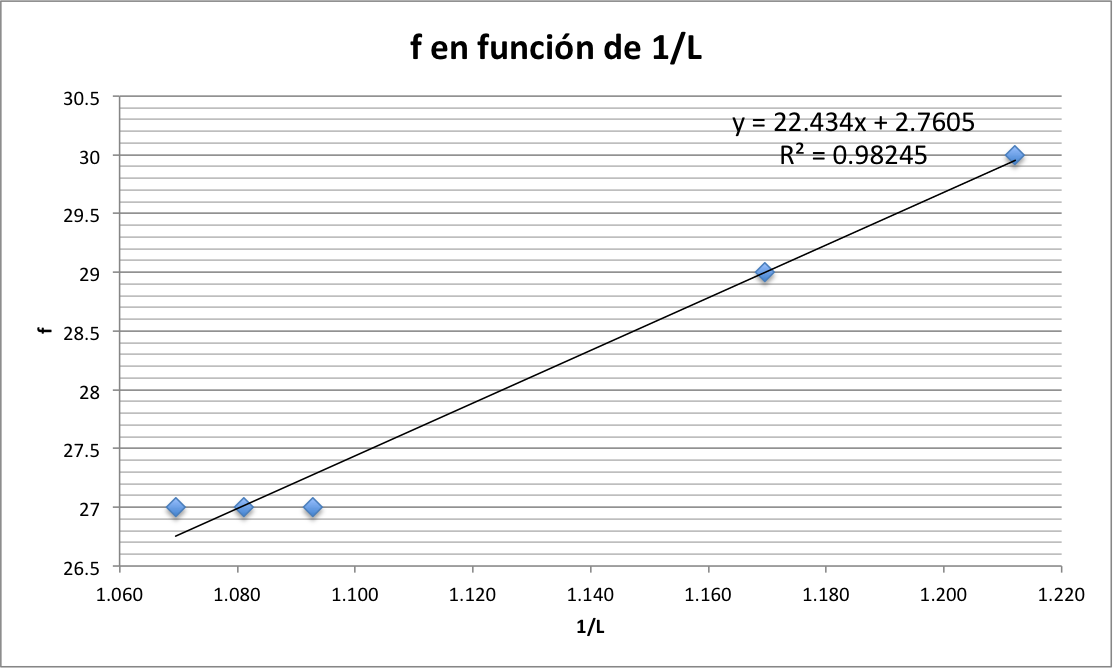
\includegraphics[width=1.0\textwidth]{3.png}
    \caption{Gráfica de la frecuencia en función del inverso de la longitud (L).}
    \label{fig:my_label}
\end{figure}
\emph{Solución: }
$\\$
$\\$
Al construir una gráfica de la frecuencia en función del inverso de la longitud de la cuerda su gráfica corresponde a una línea recta de la forma que muestra la ecuación $(1) \emph{(Veáse Figura 2)}$. Lo que muestra que la relación entre la frecuencia y el inverso de la longitud de la cuerda son directamente proporcionales, es decir:

\begin{equation}
    f \ \ \ \ \alpha \ \ \ \ \frac{1}{L}
\end{equation}
$\bullet$ A partir de su gráfico obtenga la ecuación que relaciona la frecuencia con la longitud de la cuerda y de esta ecuación obtenga un nuevo valor para $\mu$ con su respectiva incertidumbre. Compare este valor con el teórico.

$\\$
\emph{Solución: }
\begin{equation}
    y=22.434x+2.7605
\end{equation}

\begin{equation}
    22.434=\frac{n}{2}\sqrt{\frac{T}{\mu}}
\end{equation}

\begin{equation}
    \mu={n^{2}}\frac{T}{22.434^{2}}
\end{equation}

Para el tercer análisis se obtuvieron los valores experimentales directos de la tensión $(T)$ y del segundo armonico $(n)$
\begin{equation*}
    T=1.8865 (N) \ \ \ \ \ \ n=2 
\end{equation*}

\begin{equation}
    \mu=3.748x10^{-03}\pm 0.001 \frac{kg}{m}
\end{equation}

\begin{equation}
    \%E=\frac{|3.7x10^{-03}-3.748x10^{-03}|}{3.7x10^{-03}}x100\%=1.29\%
\end{equation}


\subsection{}
De los resultados obtenidos, diga cuál de los valores de $\mu$ es el más cercano al valor real. De una justificación a su resultado. 
$\\$
$\\$
\emph{Solución:}
$\\$
De acuerdo a los resultados obtenidos y a las gráficas de las relaciones entre las variables, la que más se acerca al valor real de la densidad de masa lineal $\mu$ es la relación entre la frecuencia $f$ y el inverso de la longitud de la cuerda $\frac{1}{L}$. Esto se debe a que el valor de la pendiente $m$ es un valor de correlación muy aproximado entre las variables y me describe el comportamiento de la densidad como un valor muy aproximado al valor real o teórico. 
$\\$
La otras relaciones no nos aproximaron de forma eficaz al valor real y no permitieron que el análisis de los resultados fuera acorde por el planteado a nivel teórico.

\section{Conclusiones}
$\\$
$\bullet$ En este laboratorio através de la toma de datos y la variación de los parámetros que describen el comportamiento de la oscilaciones en una cuerda tensa, se pudo establecer una correspondencia entre los paramétros en función de la frecuencia.  

$\bullet$ En la elaboración del análisis se pudo establecer un criterío para desarrollar métodos de toma de datos, basados en las incertumbres que describe cada variable.

$\bullet$ Este laboratorio aborda las oscilaciones que se dan en una cuerda tensa, un primer acercamiento a los sistemas oscilatorios y la mécanica lagragiana de la interacción entre los cuerpos.

\section{Bibliografia}

[1] \ \ Oscilaciones en una cuerda tensa (2013), Universidad Tecnológica de Pereira. Tomado de: $http://media.utp.edu.co/facultad-ciencias-basicas \\ /archivos/contenidos-departamento-de-fisica/experimento9if.pdf$
$\\$
$\\$
[2] \ \ Oscilaciones en una cuerda tensa (2012), Universidad Nacional de San Luis, Argentina. Tomado de: $http://linux0.unsl.edu.ar/~hvelasco/ \\
velasco3/DOCS/LAB/Lab_Fisica_7.pdf$


\section{Apéndice}
\subsection{Tablas de datos}

\begin{table}[h!]
\centering
\begin{tabular}{ |c|c| } 
 \hline
 n & f (Hz) \\ 
 \hline
 1 & 11 \\ 
 2 & 21 \\  
 3 & 31 \\  
 4 & 43 \\ 
 5 & 54 \\  
 \hline
\end{tabular}
\caption{Frecuencia en función de el numero de armónicos}
\label{table:1}
\end{table}


\begin{table}[h!]
\centering
\begin{tabular}{ |c|c|c|c| } 
 \hline
 n & f (Hz) & T & $\sqrt{T}$ \\ 
 \hline
 2 & 24 & 1.89 & 1.37 \\ 
 2 & 22 & 1.65 & 1.29 \\  
 2 & 20 & 1.42 & 1.19 \\  
 2 & 18 & 1.19 & 1.09 \\ 
 2 & 16 & 0.46 & 0.68 \\  
 \hline
\end{tabular}
\caption{Frecuencia en función de la raíz cuadrada de la tensión}
\label{table:1}
\end{table}

\begin{table}[h!]
\centering
\begin{tabular}{ |c|c|c|c| } 
 \hline
 n & f (Hz) & L(m) & $\frac{1}{L}$ $\frac{1}{m}$\\ 
 \hline
 2 & 27 & 0.94 & 1.070 \\ 
 2 & 30 & 0.83 & 1.212 \\  
 2 & 27 & 0.93 & 1.081 \\  
 2 & 29 & 0.86 & 1.170 \\ 
 2 & 27 & 0.92 & 1.093 \\  
 \hline
\end{tabular}
\caption{Frecuencia en función del inverso de la longitud de la cuerda}
\label{table:1}
\end{table}

\subsection{Calculo de las incertidumbres}
\subsubsection{Incertidumbre para medidas indirectas}
$\bullet$ Especificar el mensurando:
\begin{equation}
    Y=f(X_{1},X_{2},...,X_{n})
\end{equation}
donde 
\begin{equation*}
    Y \ \ \ \ \ \ Es \ el \ mensurando
\end{equation*}
\begin{equation*}
    f \ \ \ Es \ la \ funcion \ que \ relaciona \ la \
    magnitud \ medida \ con \ los \ factores \ que \ la \ afectan 
\end{equation*}
\begin{equation*}
    X_{1},X_{2},...,X_{n} \ \ \ \ \ \ Son \ las \ magnitudes \ de \ entrada
\end{equation*}

$\bullet$ Para nuestro caso tenemos:
\begin{equation*}
    f_{n}=\frac{n}{2L}\sqrt{\frac{T}{\mu}}
\end{equation*}
\begin{equation*}
    y=mx\pm b
\end{equation*}

$\bullet$ Estimar la incertidumbre combinada y los grados de libertad de todas las magnitudes directas que intervienen en el cálculo de la mágnitud de interés:

$\\$
$\\$
$\bullet$ Calcular los coeficientes de sensibilidad: 
\begin{equation}
    C_{i}=\frac{\partial f}{\partial x_{i}}
\end{equation}

Para nuestro primer caso tenemos:
\begin{equation}
    C_{n}=\frac{1}{2L}\sqrt{\frac{T}{\mu}}
\end{equation}

Para nuestro segundo caso tenemos:
\begin{equation}
    C_{T}=\frac{n}{4L}\frac{1}{\sqrt{\mu T}}
\end{equation}

Para nuestro tercer caso tenemos:
\begin{equation}
    C_{L}=-\frac{n}{4L^{2}}\sqrt{\frac{T}{\mu}}
\end{equation}

$\bullet$ Determinar si las magnitudes de entrada están correlacionadas:

$\\$
$\\$

$\bullet$ Calcular la incertidumbre combinada
\begin{equation}
    u_{c}=\sqrt{\sum_{i=1}^{n}C_{i}^{2}u^{2}(X_{i})}
\end{equation}

\emph{Nota:} El resultado de los pasos anteriores se realizarón en el programa Microsoft EXCEL y se adjuntan en la entrega del informe.

\end{document}

